\chapter{Embodiment Design}
The next phase in the design methodology is embodiment design. This phase, as defined by Pahl and Beitz \cite[227]{Pahl2007}, involves starting with the fundamental solution or concept for a technical product and then advancing the design in alignment with technical and economic criteria, taking into account further information. The ultimate objective is to reach a stage where the subsequent detailed design can smoothly progress into the production phase. Figure \ref{fig:embodiment_design} shows the steps involved in this phase.

\begin{figure}
    \centering
    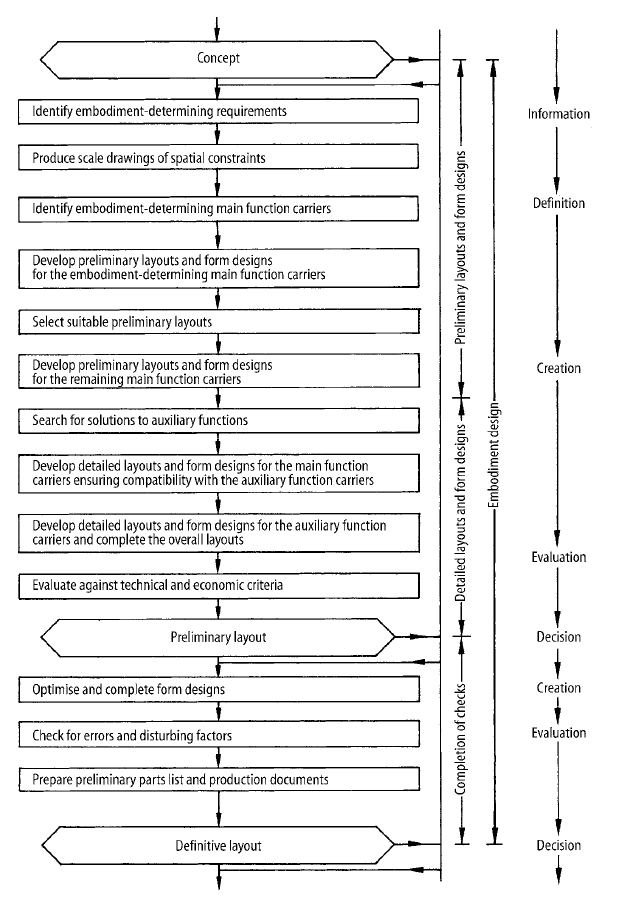
\includegraphics[width=0.92\linewidth]{texs/Part1/chapter4/image/embodiment.png}
    \caption{Steps in Embodiment Design \cite[229]{Pahl2007}}
    \label{fig:embodiment_design}
\end{figure}

\section{Basic Rules of Embodiment Design}
Regarding product design, some basic rules must be followed. As defined by Pahl and Beitz \cite[234-235]{Pahl2007}, they include clarity, simplicity, and safety. Neglecting these rules can potentially result in issues and accidents. Subsequent sections will provide a comprehensive exploration of these guidelines.

\subsection{Clarity}
Clarity, as described by Pahl and Beitz \cite[235]{Pahl2007}, includes establishing clear and unambiguous connections within a design, ensuring straightforward relationships between subfunctions, inputs, and outputs to prevent confusion or misinterpretation.

They also mention that clarity applies to the broader design structure, whether it involves multiple working principles or component combinations. It mandates that the design facilitates the orderly flow of energy, materials, and signals, preventing adverse effects like excessive forces or wear.

\subsection{Simplicity}
As defined by Pahl and Beitz \cite[242]{Pahl2007}, simplicity in design is characterized by an uncomplicated and easily understandable approach, often achievable by using fewer components. Such simplicity can save costs, reduce wear and tear, and minimize maintenance requirements. Nonetheless, striking a balance is crucial, as certain functions inherently demand a minimum number of components.

\subsection{Safety}
According to Pahl and Beitz \cite[247]{Pahl2007}, safety considerations are crucial in ensuring both the adequate performance of technical functions and the protection of people and the environment. Designers rely on a safety methodology outlined in the German industry standard DIN 31 000, encompassing three levels: direct safety, indirect safety, and warnings. Designers should prioritize direct safety measures, seeking solutions that inherently eliminate potential dangers. Only when this is not feasible should they resort to indirect safety measures involving the construction of specialized protective systems.

Warnings highlighting dangers and hazard zones are best utilized in conjunction with direct and indirect safety measures, clarifying specific risks. As designers address technical challenges, they encounter various constraints, not all of which can be simultaneously overcome. However, their objective remains to develop solutions that come as close as possible to meeting all requirements. It is important to note that exceptionally high safety demands can complicate design, potentially diminishing clarity and economic viability and possibly leading to project abandonment.

\section{Guideline of Embodiment Design}
In addition to the basic rules of embodiment design, Pahl and Beitz \cite[308]{Pahl2007} also stress the importance of following a set of design guidelines to help designers meet specific requirements and constraints. For this project, the \textit{Design for production} guideline are applied.

\subsection{Design for Production}
The concept of \textit{Design for Production} outlined by Pahl and Beitz \cite[355-356]{Pahl2007} underscores the significance of factoring in the production process during the design stage. This methodology empowers designers to fine-tune production costs and timelines while maintaining the product's functionality and quality. They highlight that adhering to fundamental principles of clarity and simplicity sets designers on the correct path towards realizing this objective.

\subsubsection{Appropriate Overall Layout Design}
Pahl and Beitz \cite[355-362]{Pahl2007} mentioned that the overall layout design, derived from the function structure, influences product division into assemblies and components, including sourcing decisions (in-house, bought-out, standard parts), production procedures, dimensions, batch sizes, joining methods, and quality control. The layout can lead to differential, integral, composite, or building-block construction methods.

\textit{Differential Construction} involves breaking down components into quickly produced parts, facilitating adaptability, increased component batch sizes, and more accessible quality assurance. However, it demands more outstanding machining and assembly costs and may have functional limitations due to joints.

\textit{Integral Construction} combines multiple parts into a single component, usually utilized for product optimization. It can greatly reduce cost for assembly and quality control while enhancing functionality and performance. However it usually requires more complex production procedures and may be less adaptable.

\textit{Composite Construction} refers to the integration of various components, each constructed differently, into a single unit that may require additional processing. This includes scenarios like combining cast and forged parts. Moreover, it involves employing multiple methods of joining to bring together different elements simultaneously.

\textit{Building Block Construction} results from splitting components so that the parts or assemblies can be used in other products or variants, offering flexibility and cost savings. This approach is often used in modular design, where components are designed to be easily interchangeable.

\subsubsection{Appropriate Form Design of Components}
As mentioned by Pahl and Beitz \cite[362]{Pahl2007}, numerous factors influence the cost, time, and production quality. These include parameters like shapes, dimensions, surface finishes, tolerances, and fits. These choices are essential in determining production procedures, machine types, materials, in-house vs. bought-out components, and quality control measures.

Furthermore, production facilities can impact the design of features, such as dimension limitations that necessitate component division or the procurement of bought-out components. Many guidelines are available for designing appropriate component forms. The design guideline for 3D printed components is shown in Figure \ref{fig:guideline}.

\begin{figure}
    \centering
    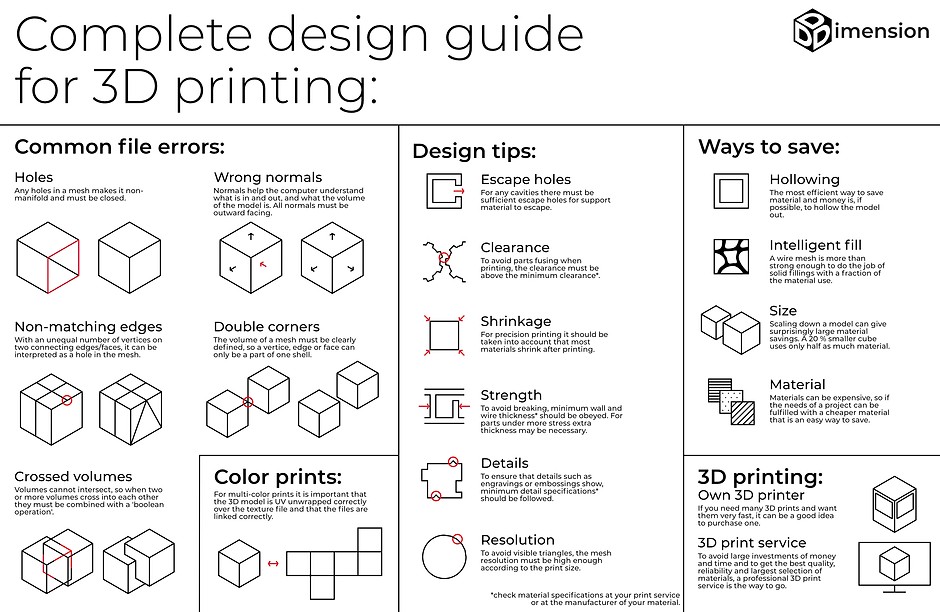
\includegraphics[width=0.92\linewidth]{texs/Part1/chapter4/image/guidelines.png}
    \caption{Design guidelines for 3D printing \cite{DDDimension_22}}
    \label{fig:guideline}
\end{figure}

\subsubsection{Appropriate Use of Standard and Bought-Out Components}
The authors advised that \cite[374-375]{Pahl2007}, designers should use readily available standard or bought-out components rather than specially produced ones to ensure favorable supply and storage conditions. Bought-out parts are often more cost-effective than in-house production. The decision between in-house or bought-out components depends on factors like production volume, market demand, costs, and available facilities. These factors may change over time, requiring periodic re-evaluation, especially for unique or batch products in heavy engineering.

\section{Preliminary Design}
In this section, we will explore multiple designs for the device. These designs are detailed 3D models of the device that we will use to evaluate their respective designs and assess their feasibility. Each of these preliminary designs will be based on the selected solution from the previous phase. Alongside the models, we will also present the production costs for each of these designs. For a more detailed breakdown of the production costs, please refer to Appendix \ref{appendix:cost-calculation}.


\subsection{Preliminary Design Variant 2}
\label{subsec:preliminary_design_variant_2}
Figure \ref{fig:preliminary_design_variant_2} showcases the 3D model of Variant 2, while Figure \ref{fig:variant2_views} provides various perspectives and body measurements of the device. The key emphasis of this design is its ergonomic shape and user-friendly attributes. With a thickness of 52.2 mm (Figure \ref{fig:variant2_right_view}), it successfully balances being slim and accommodating essential components for optimal performance.

\begin{figure}[ht!]
    \centering
    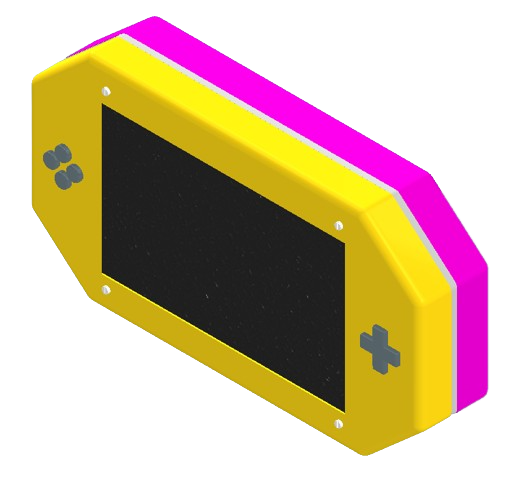
\includegraphics[height=5 cm]{texs/Part1/chapter4/image/v21.png}
    \caption{Preliminary Design Variant 2}
    \label{fig:preliminary_design_variant_2}
\end{figure}

\begin{figure}[ht!]
    \centering
    \begin{subfigure}[c]{0.65\textwidth}
        \begin{minipage}{\textwidth}
            \centering
            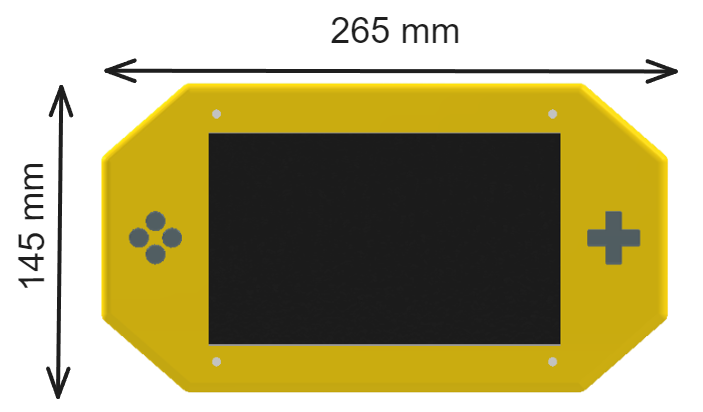
\includegraphics[height=4 cm]{texs/Part1/chapter4/image/v22.png}
        \end{minipage}
        \caption{Front View}
        \label{fig:variant2_front_view}
    \end{subfigure}
    % \hfill
    \begin{subfigure}[c]{0.25\textwidth}
        \begin{minipage}{\textwidth}
            \centering
            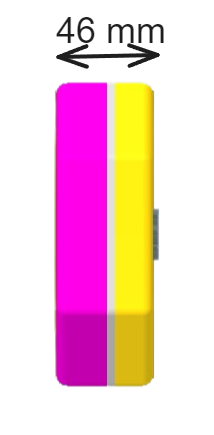
\includegraphics[height=4 cm]{texs/Part1/chapter4/image/v23.png}
        \end{minipage}
        \caption{Right View}
        \label{fig:variant2_right_view}
    \end{subfigure}
    \caption{Views of Preliminary Design Variant 2}
    \label{fig:variant2_views}
\end{figure}

\begin{figure}[ht!]
    \centering
    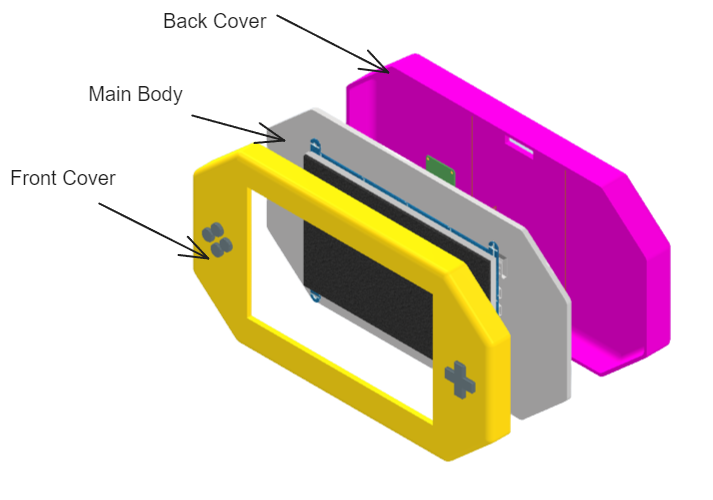
\includegraphics[width=0.5\linewidth]{texs/Part1/chapter4/image/v24.png}
    \caption{Body Components of Preliminary Design Variant 2}
    \label{fig:variant2_body_components}
\end{figure}

\begin{figure}[ht!]
    \centering
    \begin{subfigure}[c]{0.5\textwidth}
        \begin{minipage}{\textwidth}
            \centering
            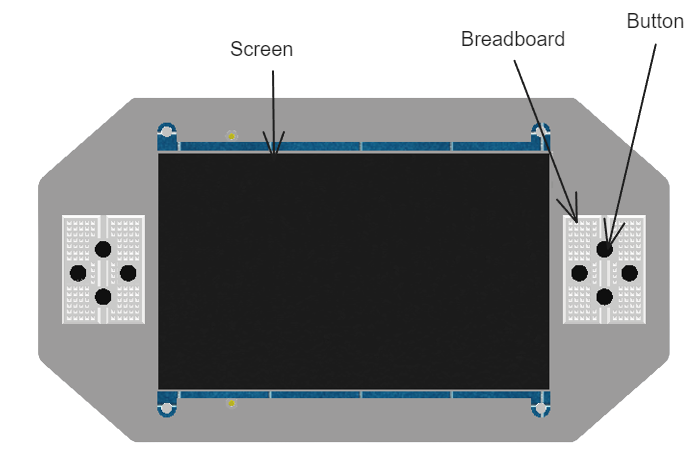
\includegraphics[height=4 cm]{texs/Part1/chapter4/image/v25.png}
        \end{minipage}
        \caption{Front View}
        \label{fig:variant2_front_view_main}
    \end{subfigure}
    % \hfill
    \begin{subfigure}[c]{0.5\textwidth}
        \begin{minipage}{\textwidth}
            \centering
            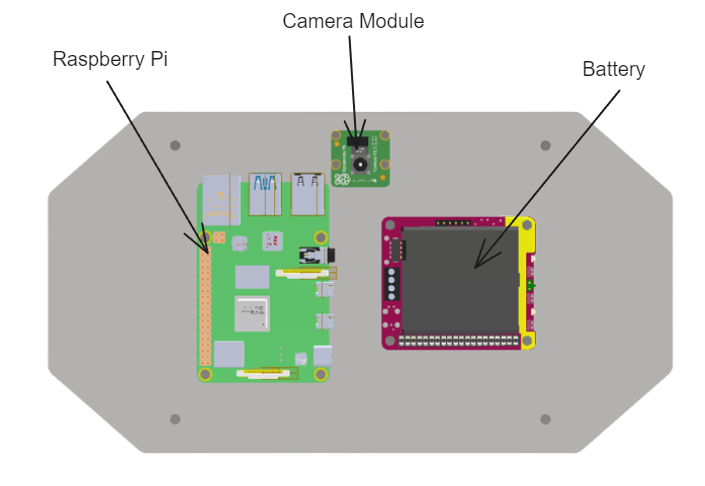
\includegraphics[height=4 cm]{texs/Part1/chapter4/image/v26.png}
        \end{minipage}
        \caption{Back View}
        \label{fig:variant2_back_view_main}
    \end{subfigure}
    \caption{Placement of inner components for Variant 2}
    \label{fig:variant2_inner_components}
\end{figure}

The physical design of Solution Variant 2 adheres to a sandwich-like structure comprising a main body, top cover, and back cover (see Figure \ref{fig:variant2_body_components}). This design choice ensures the protection of internal components and simplifies assembly and maintenance. The main body of the device functions as the central hub, accommodating the internal components and features. In contrast, the top and back covers act as protective shields, safeguarding the internal parts from any damage from external factors.

A crucial aspect of the design involves arranging internal components within the device. Following a tablet-like configuration, the main LCD is positioned on the front side of the main body, providing users with a straightforward and interactive interface (see Figure \ref{fig:variant2_front_view_main}). Simultaneously, the camera, Raspberry Pi, and battery were placed on the back side of the body (Figure \ref{fig:variant2_back_view_main}) to optimize the weight distribution and ensure a well-balanced user experience. This arrangement enhances the overall usability and convenience of the device, making it suitable for a wide range of applications.

\begin{figure}[ht!]
    \centering
    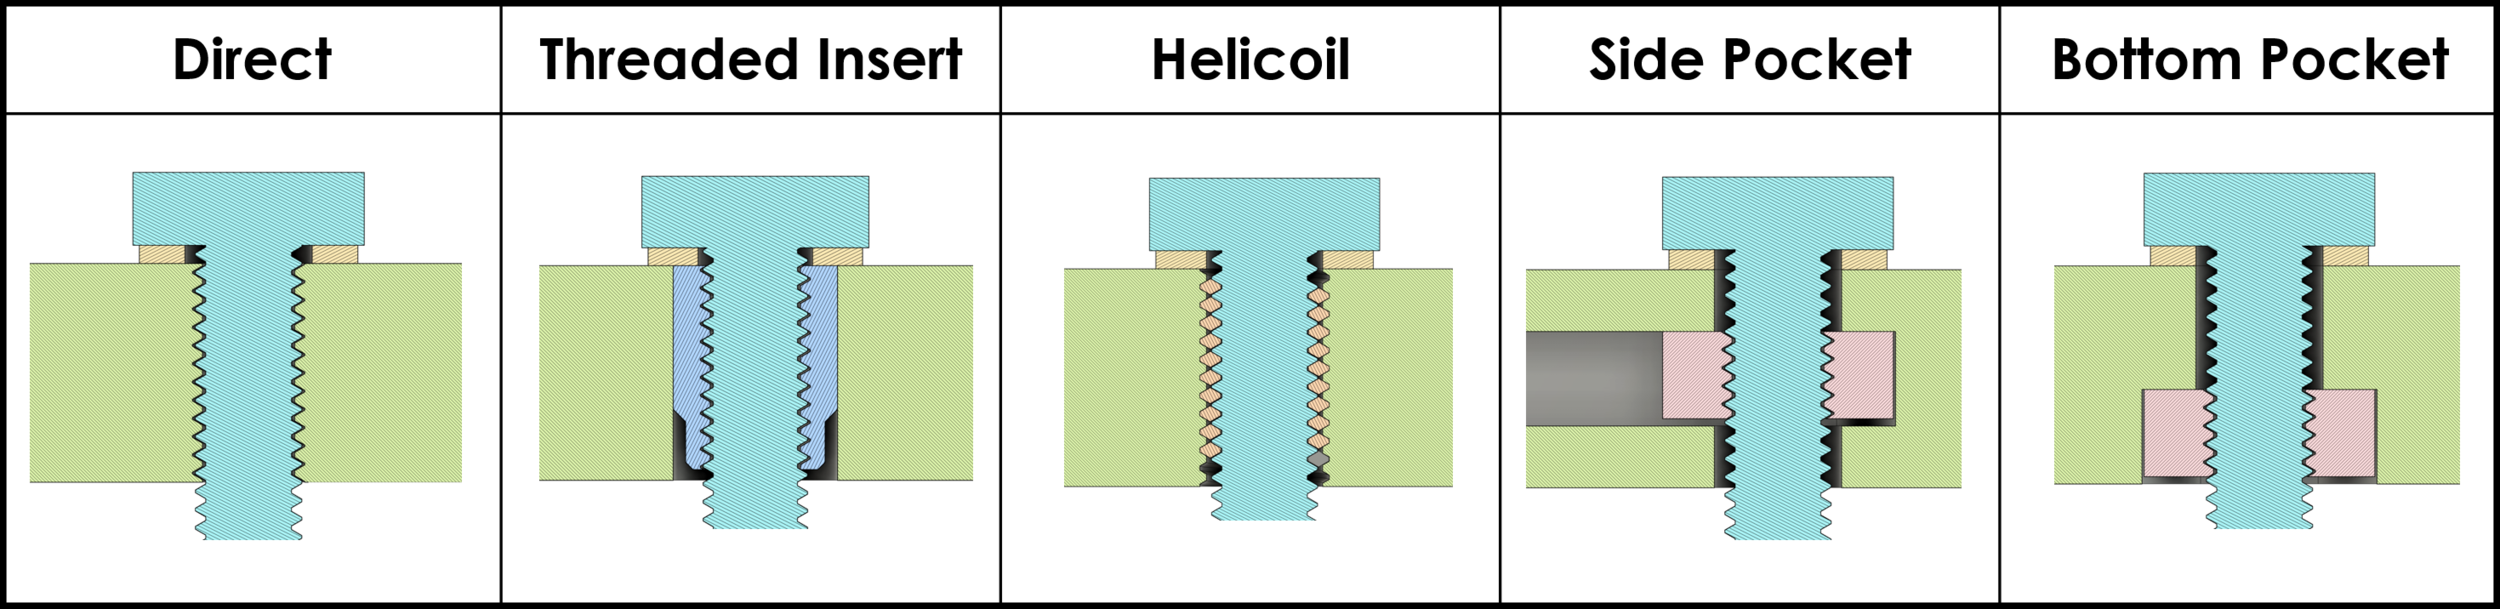
\includegraphics[width=\linewidth]{texs/Part1/chapter4/image/insert.png}
    \caption{Methods to secure 3D-printed components \cite{Hermann20}}
    \label{fig:insert}
\end{figure}

Ensuring the secure attachment of internal components to the main body is vital in the design process. Various methods of component fastening have been considered, including direct attachment, threaded inserts, helicoils, side pockets, and bottom pockets, as shown in Figure \ref{fig:insert}.

The most straightforward approach is direct attachment, in which threads are designed into a 3D-printed part to allow components to be screwed in. For more robust connections, threaded inserts can be used by designing holes in the 3D printed part and installing inserts appropriately.

Helicoils offer durable threaded holes by inserting coil-shaped inserts into the holes. Side and bottom pockets create cavities or slots in the 3D-printed part to securely hold components. Each method has its advantages and challenges. After careful evaluation, the variant opts for threaded inserts due to its simplicity and robustness.

Solution Variant 2 employs a hybrid input method combining a touch screen and physical buttons. The touch screen is oriented in landscape mode, while the buttons are positioned on either side of the screen (Figure \ref{fig:variant2_front_view}). HDMI and USB connections were established between the touch screen and Raspberry Pi to enable the integration of the touch screen. Additionally, to facilitate the functionality of the physical buttons, they are connected to Raspberry Pi using general-purpose input/output  (GPIO) pins.

\begin{figure}[ht!]
    \centering
    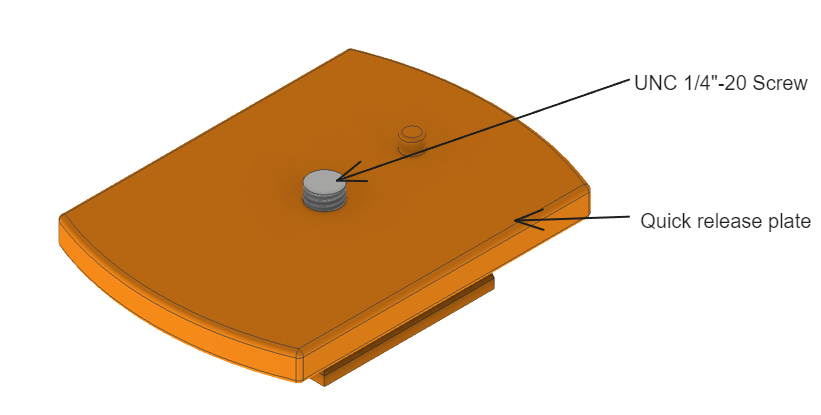
\includegraphics[height=5 cm]{texs/Part1/chapter4/image/v29.png}
    \caption{Quick release plate}
    \label{fig:variant2_quick_release_plate}
\end{figure}

In Figure \ref{fig:variant2_quick_release_plate}, we observe a quick-release plate designed to be affixed to the tripod stand. To enhance stability during usage, Solution Variant 2 can utilize a quick-release plate, which can be conveniently mounted on a tripod stand.

\subsubsection{Cost Calculation}
Table \ref{tab:printing_cost_variant_2} shows the printing cost for each component of this variant, while the total manufacturing cost is shown in Table \ref{tab:manufacturing_cost_variant_2}. In this calculation, the cost for screen, camera, and Raspberry Pi are not included, as they are used by all variants. The exclusion of these components allows for a more accurate comparison of the manufacturing costs between the variants.

\begin{table}[H]
    \centering
    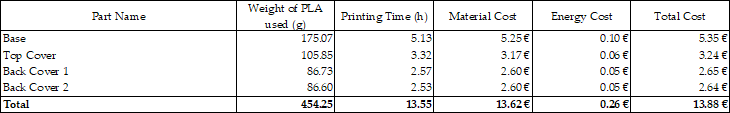
\includegraphics[width=\linewidth]{texs/Part1/chapter3/image/v2printed.png}
    \caption{Printing cost for Variant 2}
    \label{tab:printing_cost_variant_2}
\end{table}

\begin{table}[H]
    \centering
    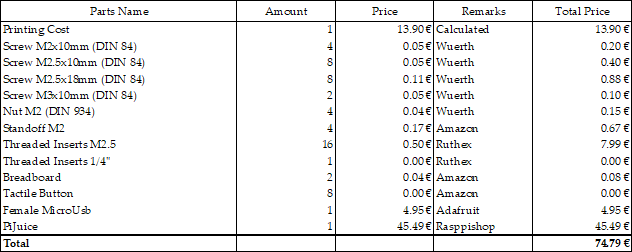
\includegraphics[width=\linewidth]{texs/Part1/chapter3/image/v2manu.png}
    \caption{Manufacturing cost for Variant 2}
    \label{tab:manufacturing_cost_variant_2}
\end{table}

\subsection{Preliminary Design Variant 3}
\label{subsec:preliminary_design_variant_3}
Variant 3 maintains a similar component arrangement to variant 2, with the screen at the front and the camera, Raspberry Pi, and battery at the rear, as shown in Figure \ref{fig:variant3_inner_components}. However, Variant 3 introduced significant changes with different screen orientations and battery types.

\begin{figure}[!ht]
    \centering
    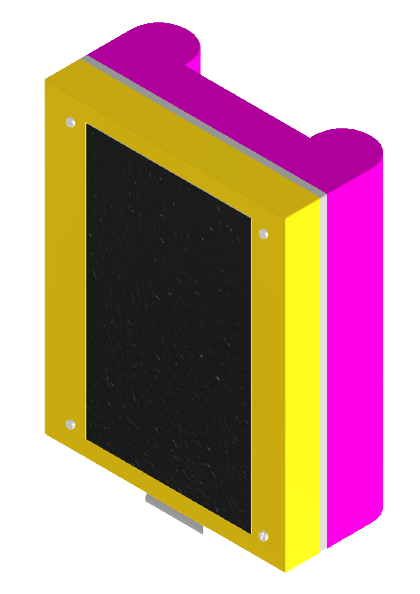
\includegraphics[height=5 cm]{texs/Part1/chapter4/image/v31.png}
    \caption{Preliminary Design Variant 3}
    \label{fig:preliminary_design_variant_3}
\end{figure}

\begin{figure}[!ht]
    \centering
    \begin{subfigure}[c]{0.47\textwidth}
        \begin{minipage}{\textwidth}
            \centering
            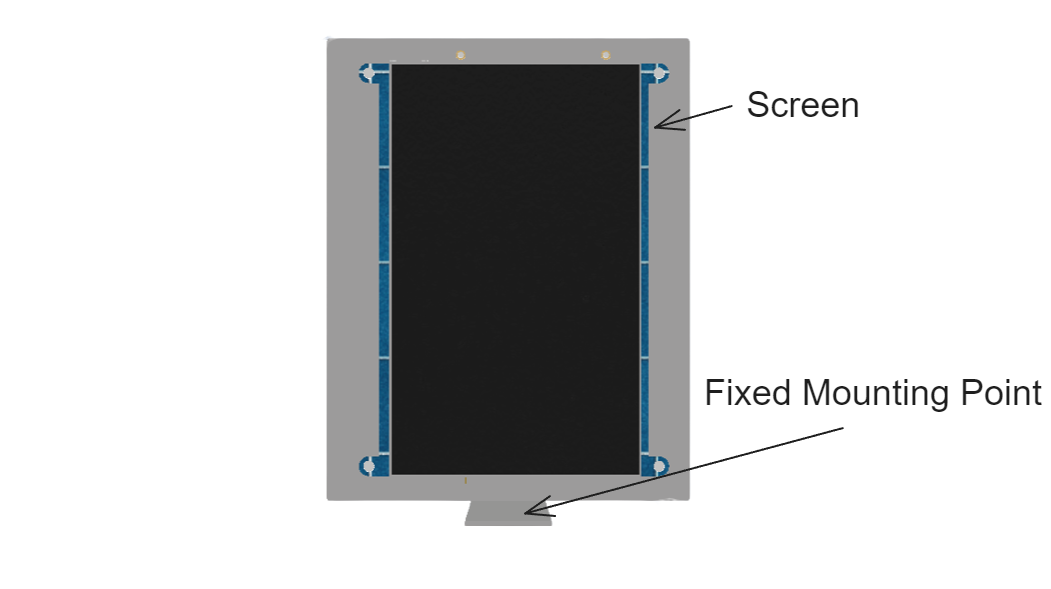
\includegraphics[height=3.8 cm]{texs/Part1/chapter4/image/v32.png}
        \end{minipage}
        \caption{Front View}
        \label{fig:variant3_front_components}
    \end{subfigure}
    % \hfill
    \begin{subfigure}[c]{0.47\textwidth}
        \begin{minipage}{\textwidth}
            \centering
            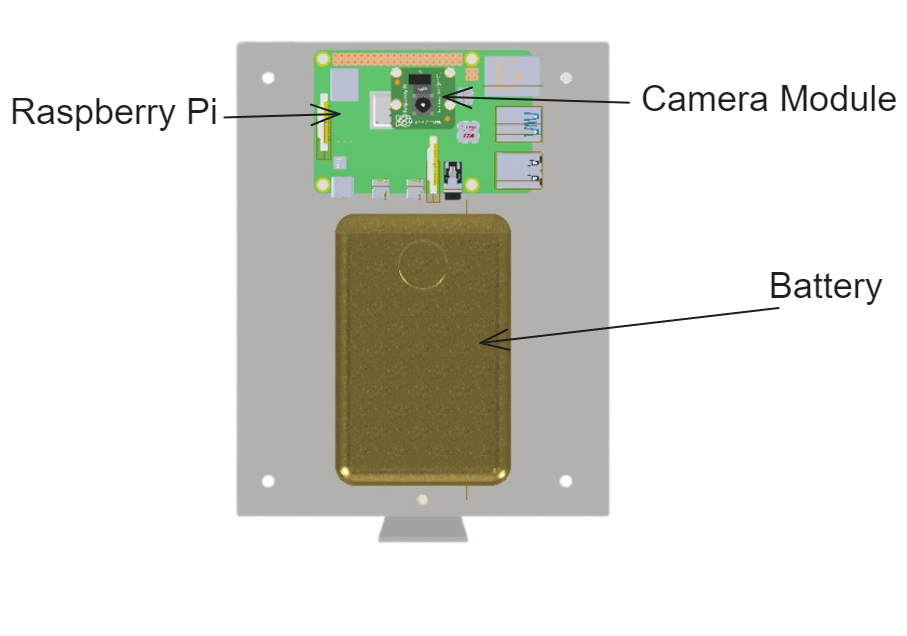
\includegraphics[height=3.8 cm]{texs/Part1/chapter4/image/v33.png}
        \end{minipage}
        \caption{Back View}
        \label{fig:variant3_back_components}
    \end{subfigure}
    \caption{Placement of inner components for Variant 3}
    \label{fig:variant3_inner_components}
\end{figure}

A noteworthy alteration is the inclusion of bumps on the back cover to enhance the ergonomics (Figure \ref{fig:variant3_bumps}). This adjustment aims to provide a more comfortable grip, improve user engagement, and extend usability. In addition, the tactile bump is added to increase handling stability of the device, ensuring that the device fits snugly in the user's hand, further enhancing the overall user experience.

\begin{figure}[!ht]
    \centering
    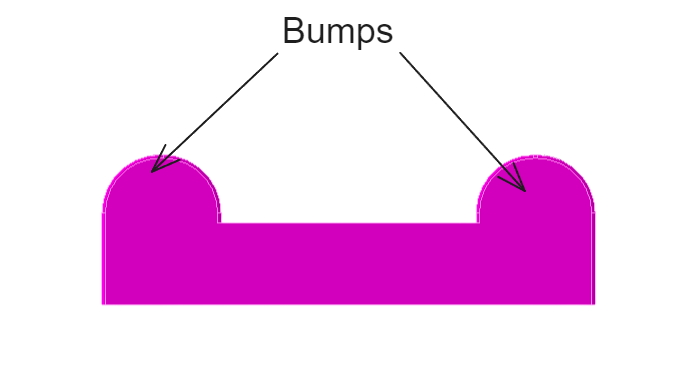
\includegraphics[width=0.5\linewidth]{texs/Part1/chapter4/image/v34.png}
    \caption{Bumps on the back cover}
    \label{fig:variant3_bumps}
\end{figure}

Variant 3 shifted from the standard battery position in variant 2, with a more noticeable difference in battery placement. Figure \ref{fig:variant3_battery_placement} illustrates a designated slot within the back cover, strategically designed to house a power bank outside the body. This configuration enhances the operational stability and simplifies the battery replacement process.

\begin{figure}[!ht]
    \centering
    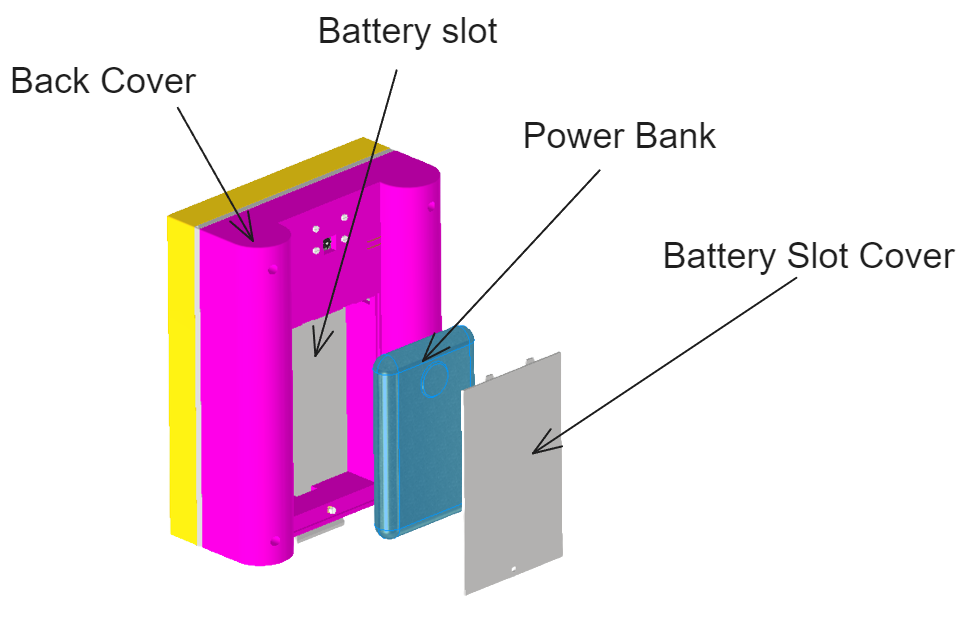
\includegraphics[width=0.5\linewidth]{texs/Part1/chapter4/image/v35.png}
    \caption{Battery Placement}
    \label{fig:variant3_battery_placement}
\end{figure}

The input methodology was streamlined using a touch screen as the sole interface. This approach simplifies the user experience by eliminating the need for physical buttons and seamlessly integrating screen interactions. Additional information regarding integrating the touchscreen with the Raspberry Pi is provided in Section \ref{subsec:preliminary_design_variant_2}.

Figure \ref{fig:variant3_front_components} shows the position of the mounting point of on the main body in Variant 3. This strategic design allows the mounting point to serve as a sturdy anchor for the device when used in a tripod stand.


\subsubsection{Cost Calculation}
Table \ref{tab:printing_cost_variant_3} shows the printing cost for each component of this variant, while the total manufacturing cost is shown in Table \ref{tab:manufacturing_cost_variant_3}.

\begin{table}[H]
    \centering
    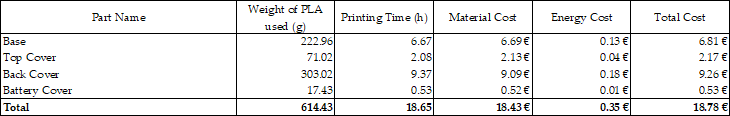
\includegraphics[width=\linewidth]{texs/Part1/chapter3/image/v3printed.png}
    \caption{Printing cost for Variant 3}
    \label{tab:printing_cost_variant_3}
\end{table}

\begin{table}[H]
    \centering
    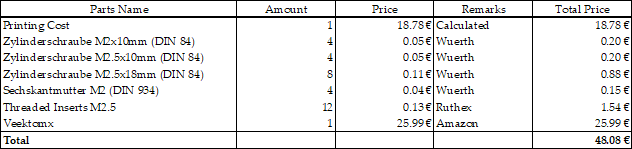
\includegraphics[width=\linewidth]{texs/Part1/chapter3/image/v3manu.png}
    \caption{Manufacturing cost for Variant 3}
    \label{tab:manufacturing_cost_variant_3}
\end{table}

\subsection{Preliminary Design Variant 6}
\label{subsec:preliminary_design_variant_6}
Figure \ref{fig:preliminary_design_variant_6} provides a detailed and comprehensive overview of the initial design concept of Variant 6. This version stands out by organizing its internal components into a configuration resembling a point-of-service (POS) system. This change from previous iterations purposefully positions the screen at an inclined angle, enhancing user interaction and optimizing the screen visibility (Figure \ref{fig:variant6_inner_components}).

\begin{figure}[!ht]
    \centering
    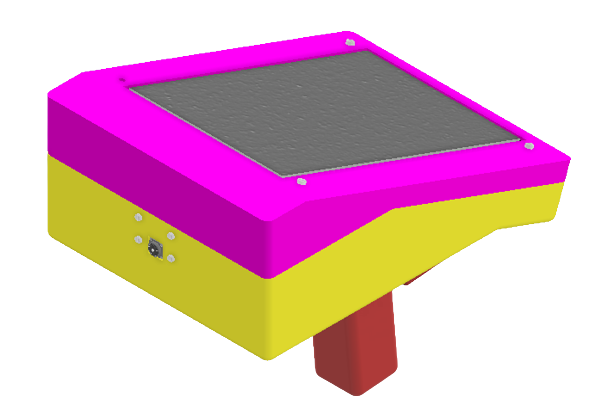
\includegraphics[height=5 cm]{texs/Part1/chapter4/image/v61.png}
    \caption{Preliminary Design Variant 6}
    \label{fig:preliminary_design_variant_6}
\end{figure}

\begin{figure}[!ht]
    \centering
    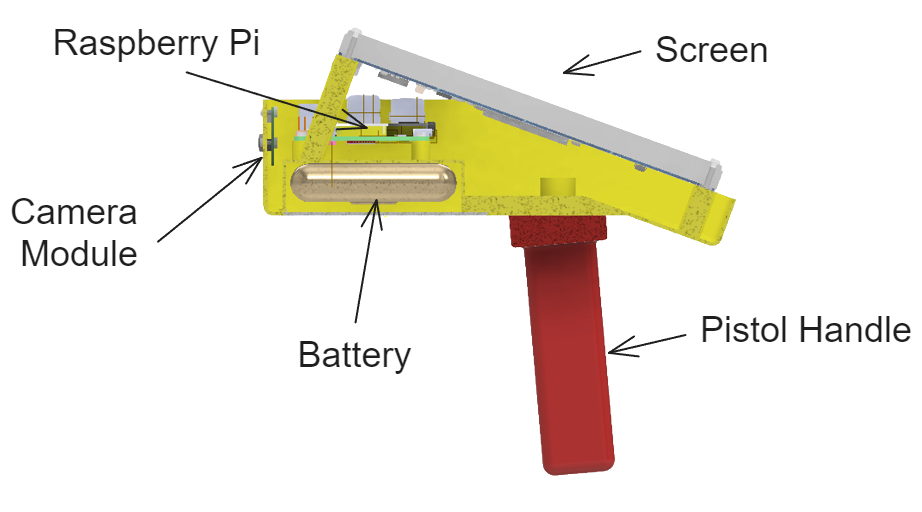
\includegraphics[height=5 cm]{texs/Part1/chapter4/image/v62.png}
    \caption{Placement of inner components for Variant 3}
    \label{fig:variant6_inner_components}
\end{figure}

Figure \ref{fig:variant6_handle_grip} demonstrates the handle grip design, while Figure \ref{fig:variant6_handle_grip_main_body} illustrates its placement on the main body. This ergonomic addition ensures a secure and comfortable hold during operation. Additionally, the handling of the device can be easily switched between the quick-change plate and the handle grip, providing users with flexible options for different scenarios (see Figure \ref{fig:variant6_quick_release_plate_main_body}).

\begin{figure}[!ht]
    \centering
    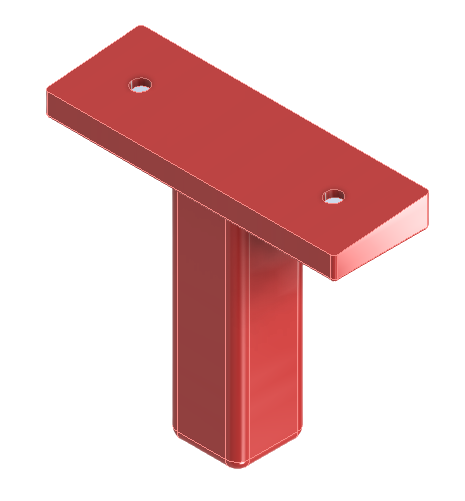
\includegraphics[width=0.5\linewidth]{texs/Part1/chapter4/image/v65.png}
    \caption{Handle Grip}
    \label{fig:variant6_handle_grip}
\end{figure}

\begin{figure}[!ht]
    \centering
    \begin{subfigure}[c]{0.47\textwidth}
        \begin{minipage}{\textwidth}
            \centering
            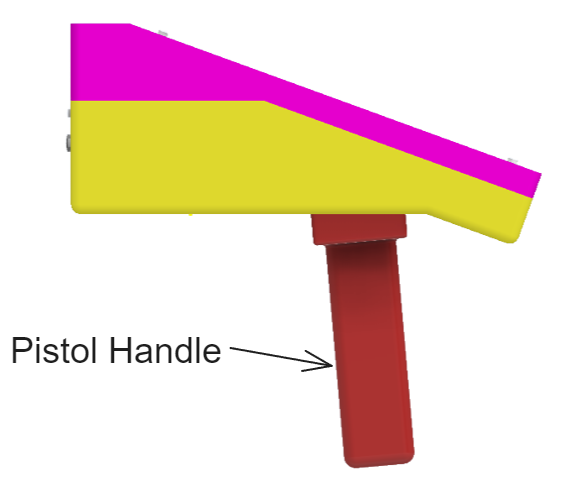
\includegraphics[height=4 cm]{texs/Part1/chapter4/image/v63.png}
        \end{minipage}
        \caption{Handle Grip with Main Body}
        \label{fig:variant6_handle_grip_main_body}
    \end{subfigure}
    % \hfill
    \begin{subfigure}[c]{0.5\textwidth}
        \begin{minipage}{\textwidth}
            \centering
            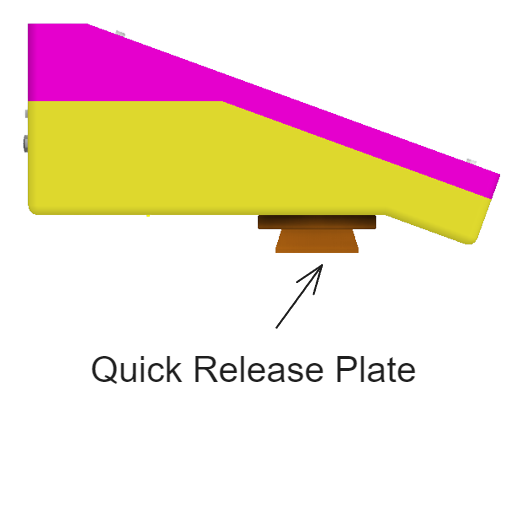
\includegraphics[height=4 cm]{texs/Part1/chapter4/image/v64.png}
        \end{minipage}
        \caption{Quick Release Plate with Main Body}
        \label{fig:variant6_quick_release_plate_main_body}
    \end{subfigure}
    \caption{Placement of handle grip and quick release plate}
    \label{fig:variant6_handle_grip_quick_release_plate}
\end{figure}

This variant boasts the same input method and battery placement as Variant 3. Please refer to Section \ref{subsec:preliminary_design_variant_3} for a comprehensive explanation.

\subsubsection{Cost Calculation}
Table \ref{tab:printing_cost_variant_6} shows the printing cost for each component of this variant, while the total manufacturing cost is shown in Table \ref{tab:manufacturing_cost_variant_6}.

\begin{table}[H]
    \centering
    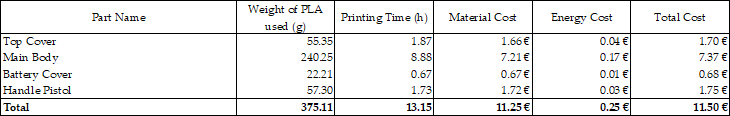
\includegraphics[width=\linewidth]{texs/Part1/chapter3/image/v6printed.png}
    \caption{Printing cost for Variant 6}
    \label{tab:printing_cost_variant_6}
\end{table}

\begin{table}[H]
    \centering
    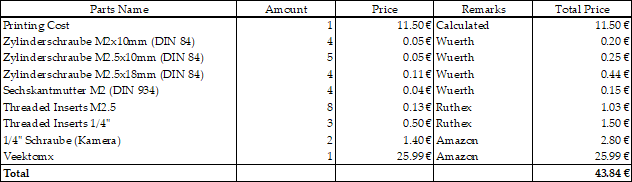
\includegraphics[width=\linewidth]{texs/Part1/chapter3/image/v6manu.png}
    \caption{Manufacturing cost for Variant 6}
    \label{tab:manufacturing_cost_variant_6}
\end{table}

\subsection{Preliminary Design Variant 7}
In Figure \ref{fig:preliminary_design_variant_7}, we can observe a 3D model for variant 7, which draws inspiration from handheld PCs. The design showcases the integration of Raspberry Pi at the back of the screen, creating a compact and unified structure, while the battery is positioned next to the screen.

\begin{figure}[!ht]
    \centering
    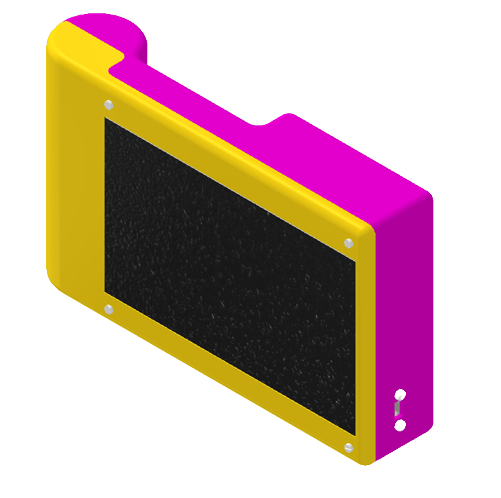
\includegraphics[height=5 cm]{texs/Part1/chapter4/image/v71.png}
    \caption{Preliminary Design Variant 7}
    \label{fig:preliminary_design_variant_7}
\end{figure}

\begin{figure}[!ht]
    \centering
    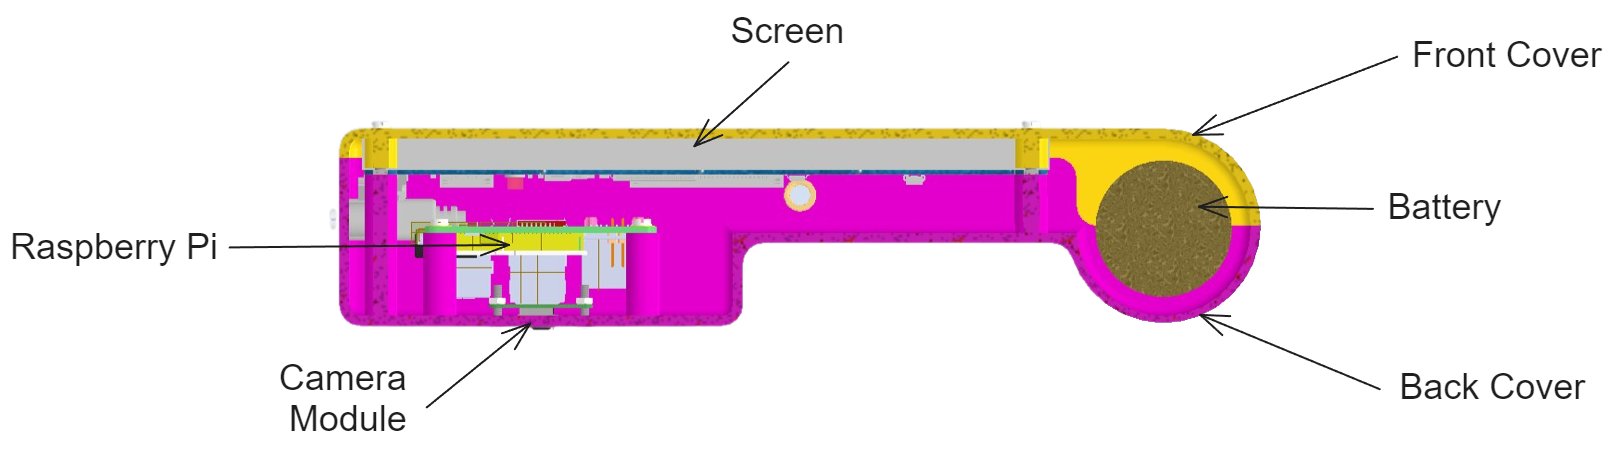
\includegraphics[height=3 cm]{texs/Part1/chapter4/image/v72.png}
    \caption{Placement of inner components for Variant 7}
    \label{fig:variant7_inner_components}
\end{figure}

\begin{figure}[!ht]
    \centering
    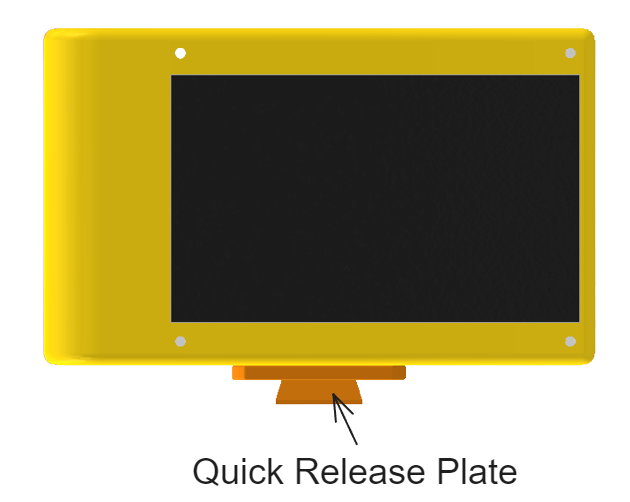
\includegraphics[height=5 cm]{texs/Part1/chapter4/image/v73.png}
    \caption{Placement of quick release plate}
    \label{fig:variant7_quick_release_plate}
\end{figure}

This design includes a bump on the side, enhancing ergonomics as shown in Figure \ref{fig:variant7_inner_components}. As with variants 2 and 6, this variant employs a quick-release plate, facilitating integration with a tripod stand. The placement of the plate can be observed in Figure \ref{fig:variant7_quick_release_plate}.

\subsubsection{Cost Calculation}
Table \ref{tab:printing_cost_variant_7} shows the printing cost for each component of this variant, while the total manufacturing cost is shown in Table \ref{tab:manufacturing_cost_variant_7}.

\begin{table}[H]
    \centering
    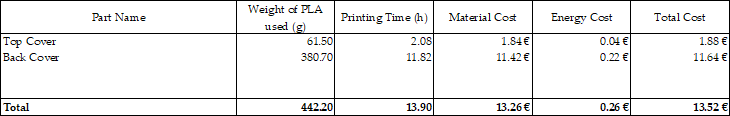
\includegraphics[width=\linewidth]{texs/Part1/chapter3/image/v7printed.png}
    \caption{Printing cost for Variant 7}
    \label{tab:printing_cost_variant_7}
\end{table}

\begin{table}[H]
    \centering
    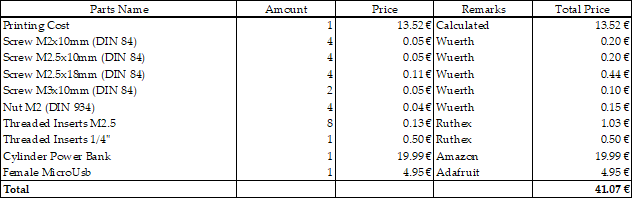
\includegraphics[width=\linewidth]{texs/Part1/chapter3/image/v7manu.png}
    \caption{Manufacturing cost for Variant 7}
    \label{tab:manufacturing_cost_variant_7}
\end{table}

\section{Evaluation with VDI 2225}
This section will evaluate the preliminary design variants using the guideline VDI 2225 \cite[109-110]{Pahl2007}. This guideline is a comprehensive framework for evaluating technical solutions based on a balanced consideration of various aspects.

The guideline advocates for comprehensive evaluation methods covering task-specific requirements and general constraints. These methods aim to quantify and qualitatively assess the properties of different variants, even in the early conceptual phase where information is limited.

The evaluation process, as discussed by Pahl and Beitz \cite[110-124]{Pahl2007}, involves several key steps:

\subsubsection{Identifying Evaluation Criteria}
This initial step involves defining a set of objectives from which specific evaluation criteria can be derived. These objectives should comprehensively cover decision-relevant requirements and general constraints, ensuring no crucial criteria are overlooked. The objectives should also be as independent as possible and expressed in quantitative or qualitative terms.

The following are the evaluation criteria for the preliminary design variants:

\textbf{Weight Distribution:} The weight distribution is evaluated by measuring the distance between the center of gravity and the point of handling. The point of handling is defined as the point where the user holds the device. A lower distance signifies a more balanced weight distribution, enhancing the user experience. The position of the center of gravity is retrieved from Computer-Aided Design (CAD) models through detailed analysis of the device's structural layout and component placement.

\textbf{Device Weight:} Device weight evaluates the overall heaviness of the equipment. A lighter device is generally easier to handle and transport, reducing user fatigue and enabling greater mobility while maintaining performance and durability. The value for device weight is calculated from CAD models by summing the individual weights of all components, materials, and structural elements that constitute the device.

\textbf{Device Size:} The size criterion considers the device's physical dimensions, assessing its compactness and portability. An optimal device size allows for convenient storage, transportation, and operation in various environments without compromising functionality. The evaluation of device size involves measuring key dimensions such as length, width, height, and any protrusions or extensions.

\textbf{Ease of Assembly:} This criterion evaluates the ease of assembling and disassembling the device. Quick and easy assembly and disassembly saves time and increases user convenience, reducing the risk of errors. Evaluation is done by counting the components used in assembly and disassembly. Fewer components often mean a more straightforward and more user-friendly design. The type and number of fasteners, such as screws or connectors, needed for assembly are also considered.

\textbf{Swappable Parts:} Swappable components refer to the ease with which parts can be interchanged or substituted. This design enhances flexibility, maintenance, and adaptability. The presence of swappable parts encourages component modularity, enabling streamlined repairs and upgrades. Swappable parts are assessed based on the quantity of interchangeable components and their compatibility. A higher number of swappable parts signifies a design that supports versatility and minimizes downtime for maintenance or repairs.

\subsubsection{Weighting Evaluation Criteria}
After establishing the evaluation criteria, their relative importance is assessed through weighting factors ($w$). This step is crucial in eliminating less significant criteria before the actual evaluation. Weightings should reflect the relative importance of each evaluation criterion.

Guideline VDI 2225 aims to avoid weightings and instead relies on criteria of roughly equal importance. However, weightings (like 2x or 3x) are used when there are significant differences between criteria.
Table \ref{tab:weighting} shows the weighting factors for the evaluation criteria.

\begin{table}[!ht]
    \centering
    \begin{tabular}{|l|c|}
        \hline
        \textbf{Criteria}   & \textbf{Weighting Factor, $w$} \\ \hline
        Weight Distribution & 3x                             \\ \hline
        Device Weight       & 2x                             \\ \hline
        Device Size         & 1x                             \\ \hline
        Ease of Assembly    & 1x                             \\ \hline
        Swappable Parts     & 2x                             \\ \hline
    \end{tabular}
    \caption{Weighting Factors for Evaluation Criteria}
    \label{tab:weighting}
\end{table}

\subsubsection{Assessing Values}
This step involves assigning values ($v_{ij}$) to the variants based on the relative scale of the determined parameters. Guideline VDI 2225 suggests using a range from 0 to 4. Table \ref{tab:value_scale} shows the scale used to evaluate the preliminary design variants. \Cref{tab:value_scale_weight_distribution,tab:value_scale_device_weight,tab:value_scale_device_size,tab:value_scale_ease_of_assembly,tab:value_scale_swappable_parts} show the value scales for the individual evaluation criteria. Equation \ref{eq:weight_calculation} shows the formula used to calculate the weighted value ($wv_{ij}$) for each variant.

\begin{table}[!ht]
    \centering
    \begin{tabular}{|c|c|}
        \hline
        \textbf{Points, $v_{ij}$} & \textbf{Meaning}  \\ \hline
        0                         & unsatisfactory    \\ \hline
        1                         & just tolerable    \\ \hline
        2                         & adequate          \\ \hline
        3                         & good              \\ \hline
        4                         & very good (ideal) \\ \hline
    \end{tabular}
    \caption{Value Scale for Evaluation \cite[115]{Pahl2007}}
    \label{tab:value_scale}
\end{table}

\begin{table}[H]
    \centering
    \begin{tabular}{|c|c|}
        \hline
        \multicolumn{2}{|c|}{\textbf{Weight Distribution}} \\ \hline
        \textbf{Range, mm} & \textbf{Point, $v_{ij}$}      \\ \hline
        0-10               & 4                             \\ \hline
        10-50              & 3                             \\ \hline
        50-100             & 2                             \\ \hline
        100-150            & 1                             \\ \hline
        $\geq$ 150         & 0                             \\ \hline
    \end{tabular}
    \caption{Value Scale for Weight Distribution}
    \label{tab:value_scale_weight_distribution}
\end{table}

\begin{table}[H]
    \centering
    \begin{tabular}{|c|c|}
        \hline
        \multicolumn{2}{|c|}{\textbf{Device Weight}} \\ \hline
        \textbf{Range, g} & \textbf{Point, $v_{ij}$} \\ \hline
        0-500             & 4                        \\ \hline
        500-1000          & 3                        \\ \hline
        1000-1500         & 2                        \\ \hline
        1500-2000         & 1                        \\ \hline
        $\geq$ 2000       & 0                        \\ \hline
    \end{tabular}
    \caption{Value Scale for Device Weight}
    \label{tab:value_scale_device_weight}
\end{table}

\begin{table}[H]
    \centering
    \begin{tabular}{|c|c|}
        \hline
        \multicolumn{2}{|c|}{\textbf{Device Size}}    \\ \hline
        \textbf{Range, mm} & \textbf{Point, $v_{ij}$} \\ \hline
        0-100              & 4                        \\ \hline
        100-200            & 3                        \\ \hline
        200-300            & 2                        \\ \hline
        300-400            & 1                        \\ \hline
        $\geq$ 400         & 0                        \\ \hline
    \end{tabular}
    \caption{Value Scale for Device Size}
    \label{tab:value_scale_device_size}
\end{table}

\begin{table}[H]
    \centering
    \begin{tabular}{|c|c|}
        \hline
        \multicolumn{2}{|c|}{\textbf{Ease of Assembly}} \\ \hline
        \textbf{Range} & \textbf{Point, $v_{ij}$}       \\ \hline
        0-25           & 4                              \\ \hline
        25-50          & 3                              \\ \hline
        50-75          & 2                              \\ \hline
        75-100         & 1                              \\ \hline
        $\geq$ 100     & 0                              \\ \hline
    \end{tabular}
    \caption{Value Scale for Ease of Assembly}
    \label{tab:value_scale_ease_of_assembly}
\end{table}

\begin{table}[H]
    \centering
    \begin{tabular}{|c|c|}
        \hline
        \multicolumn{2}{|c|}{\textbf{Swappable Parts}} \\ \hline
        \textbf{Range} & \textbf{Point, $v_{ij}$}      \\ \hline
        $\geq$ 4       & 4                             \\ \hline
        3              & 3                             \\ \hline
        2              & 2                             \\ \hline
        1              & 1                             \\ \hline
        0              & 0                             \\ \hline
    \end{tabular}
    \caption{Value Scale for Swappable Parts}
    \label{tab:value_scale_swappable_parts}
\end{table}

\begin{equation}
    wv_{ij} = w_{i} \cdot v_{ij}
    \label{eq:weight_calculation}
\end{equation}


\subsubsection{Determining the Overall Value}
The overall value of each variant ($OWV_{j}$) is calculated by summing the weighted values ($wv_{ij}$) of all evaluation criteria (see Equation \ref{eq:weighted_sum}).

\begin{equation}
    OWV_{j}=\sum_{i=1}^{n}wv_{ij}
    \label{eq:weighted_sum}
\end{equation}

\subsubsection{Comparing Concept Variants}
With the overall values ($OWV_{j}$) of the concept variants, the variants can be compared and evaluated based on their rating ($R$) which is calculated using Equation \ref{eq:total_rating}. The technical rating ($R_{t}$) is calculated using Equation \ref{eq:technical_rating}, where $v_{max}$ is the maximum value of the value scale, and $n$ is the number of evaluation criteria.

The economic rating ($R_{e}$) is calculated using Equation \ref{eq:economic_rating}, where $C_{o}$ is the comparative cost, and $C_{variant}$ is the cost of the variant. For this project, $C_{o}$ is set to be 60\% of the cost of the least expensive variant (see Equation \ref{eq:comparative_cost}).

The best variant is determined by comparing each variant's total rating ($R$). The variant with the highest total rating is considered the best variant.


\begin{equation}
    R=\frac{R_{t}+R_{e}}{2}
    \label{eq:total_rating}
\end{equation}

\begin{equation}
    R_t=\frac{OWV_{j}}{v_{max}\cdot\sum_{i=1}^{n}w_{i}}
    \label{eq:technical_rating}
\end{equation}

\begin{equation}
    R_e=\frac{C_{o}}{C_{variant}}
    \label{eq:economic_rating}
\end{equation}

\begin{equation}
    C_{o}=0.6\cdot C_{minimum}
    \label{eq:comparative_cost}
\end{equation}

\subsection{Evaluation of Preliminary Design Variant}
The result of the evaluation of the preliminary design variants will be presented in this section. Table \ref{tab:tech_eval_1} and  Table \ref{tab:tech_eval_2} shows the technical evaluation of the preliminary design variants, while Table \ref{tab:economic_eval} shows the economic evaluation of the variants. The total rating of the variants is shown in Table \ref{tab:total_rating}. Based on the total rating, Variant 6 is the best variant, followed by Variant 7, Variant 3, and Variant 2.

\begin{table}[!ht]
    \centering
    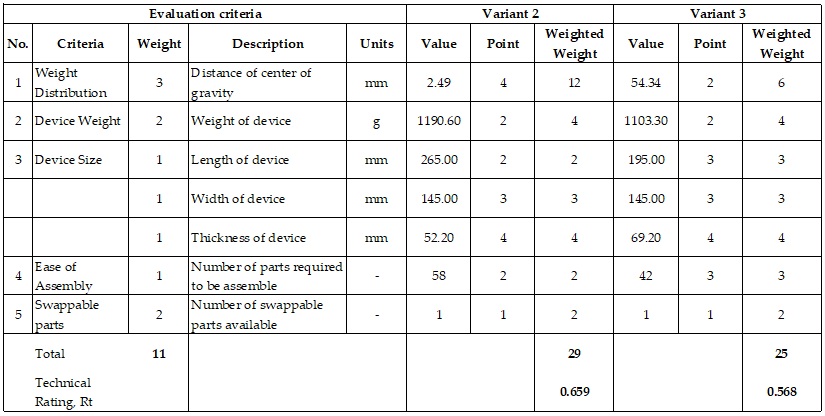
\includegraphics[width=0.95\linewidth]{texs/Part1/chapter4/image/tech_eval_1.png}
    \caption{Technical Evaluation of Preliminary Design Variants (1/2)}
    \label{tab:tech_eval_1}
\end{table}

\begin{table}[!ht]
    \centering
    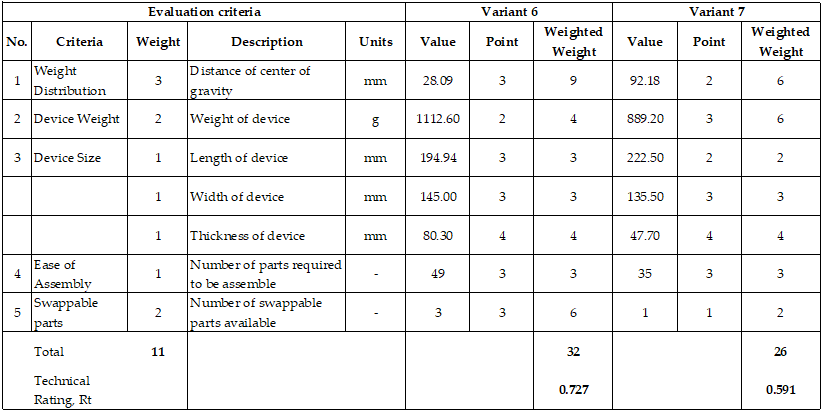
\includegraphics[width=0.95\linewidth]{texs/Part1/chapter4/image/tech_eval_2.png}
    \caption{Technical Evaluation of Preliminary Design Variants (2/2)}
    \label{tab:tech_eval_2}
\end{table}

\begin{table}[!ht]
    \centering
    \begin{tabular}{|c|c|c|}
        \hline
        \multicolumn{3}{|c|}{\textbf{Production Cost}}                                                 \\ \hline
        \textbf{Variant} & \textbf{Cost, $C_{variant}$(\texteuro)} & \textbf{Economic Rating, $R_{e}$} \\ \hline
        Variant 2        & 74.79                                   & 0.33                              \\ \hline
        Variant 3        & 48.08                                   & 0.52                              \\ \hline
        Variant 6        & 43.84                                   & 0.56                              \\ \hline
        Variant 7        & 41.07                                   & 0.60                              \\ \hline
    \end{tabular}
    \caption{Economic Evaluation of Preliminary Design Variants}
    \label{tab:economic_eval}
\end{table}

\begin{table}[!ht]
    \centering
    \begin{tabular}{|c|c|c|c|}
        \hline
        \textbf{Variant} & \textbf{Technical Rating, $R_{t}$} & \textbf{Economic Rating, $R_{e}$} & \textbf{Total Rating, $R$} \\ \hline
        Variant 2        & 0.66                               & 0.33                              & 0.494                      \\ \hline
        Variant 3        & 0.57                               & 0.51                              & 0.540                      \\ \hline
        Variant 6        & 0.73                               & 0.64                              & 0.645                      \\ \hline
        Variant 7        & 0.59                               & 0.60                              & 0.596                      \\ \hline
    \end{tabular}
    \caption{Total Rating of Preliminary Design Variants}
    \label{tab:total_rating}
\end{table}


\chapter{Detail Design}
\label{ch:detail_design}
Detail design involves finalizing the specifications of individual components, including their shapes, dimensions, materials, and surface properties \cite[436]{Pahl2007}. Figure \ref{fig:detail_design_steps} shows the steps involved in the detail design process.

\begin{figure}[!ht]
    \centering
    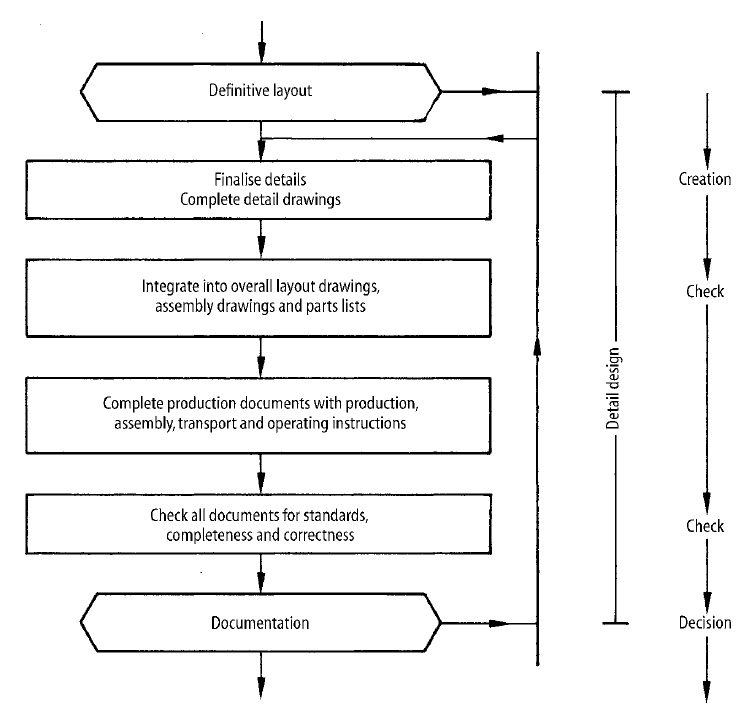
\includegraphics[width=0.95\linewidth]{texs/Part1/chapter4/image/detaildesignstep.png}
    \caption{Steps in the detail design process}
    \label{fig:detail_design_steps}
\end{figure}

Additionally, it encompasses the creation of production documents such as detailed component drawings and assembly instructions \cite[436]{Pahl2007}. CAD software often facilitates these tasks, allowing for efficient production planning and control.

The evaluation of the preliminary design variants shows that Variant 6 is the best. Hence, this variant will be used for the detailed design. Any improvements will be added to the design, while any weaknesses will be addressed. The result of this process is the final design of the device. The detailed drawing of the device is shown in Appendix \ref{appendix:cad-drawings}.

\subsubsection{Power Switch}
This component is critical in controlling the Raspberry Pi's power supply. It is imperative to have a reliable method for powering up and shutting down the Raspberry Pi to ensure smooth operation and prevent potential data corruption.

One available method utilizes the GPIO pins to initiate a shutdown sequence for the Raspberry Pi \cite{Labidi21}. While effective in bringing the device to a hibernation state, it is essential to note that this method does not completely cut off power. As a result, the Raspberry Pi still draws a minimal amount of power even in this low-power state \cite{jdb}.

A more straightforward approach is recommended to achieve more efficient power management, which involves the implementation of a simple physical push button as switch (refer to Figure \ref{fig:power_switch}). This implementation directly connects and disconnects the power supply to the Raspberry Pi. As a result, when the switch is in the \textit{off} position, it completely severs the power supply, ensuring that the Raspberry Pi consumes no power whatsoever.

\begin{figure}[!ht]
    \centering
    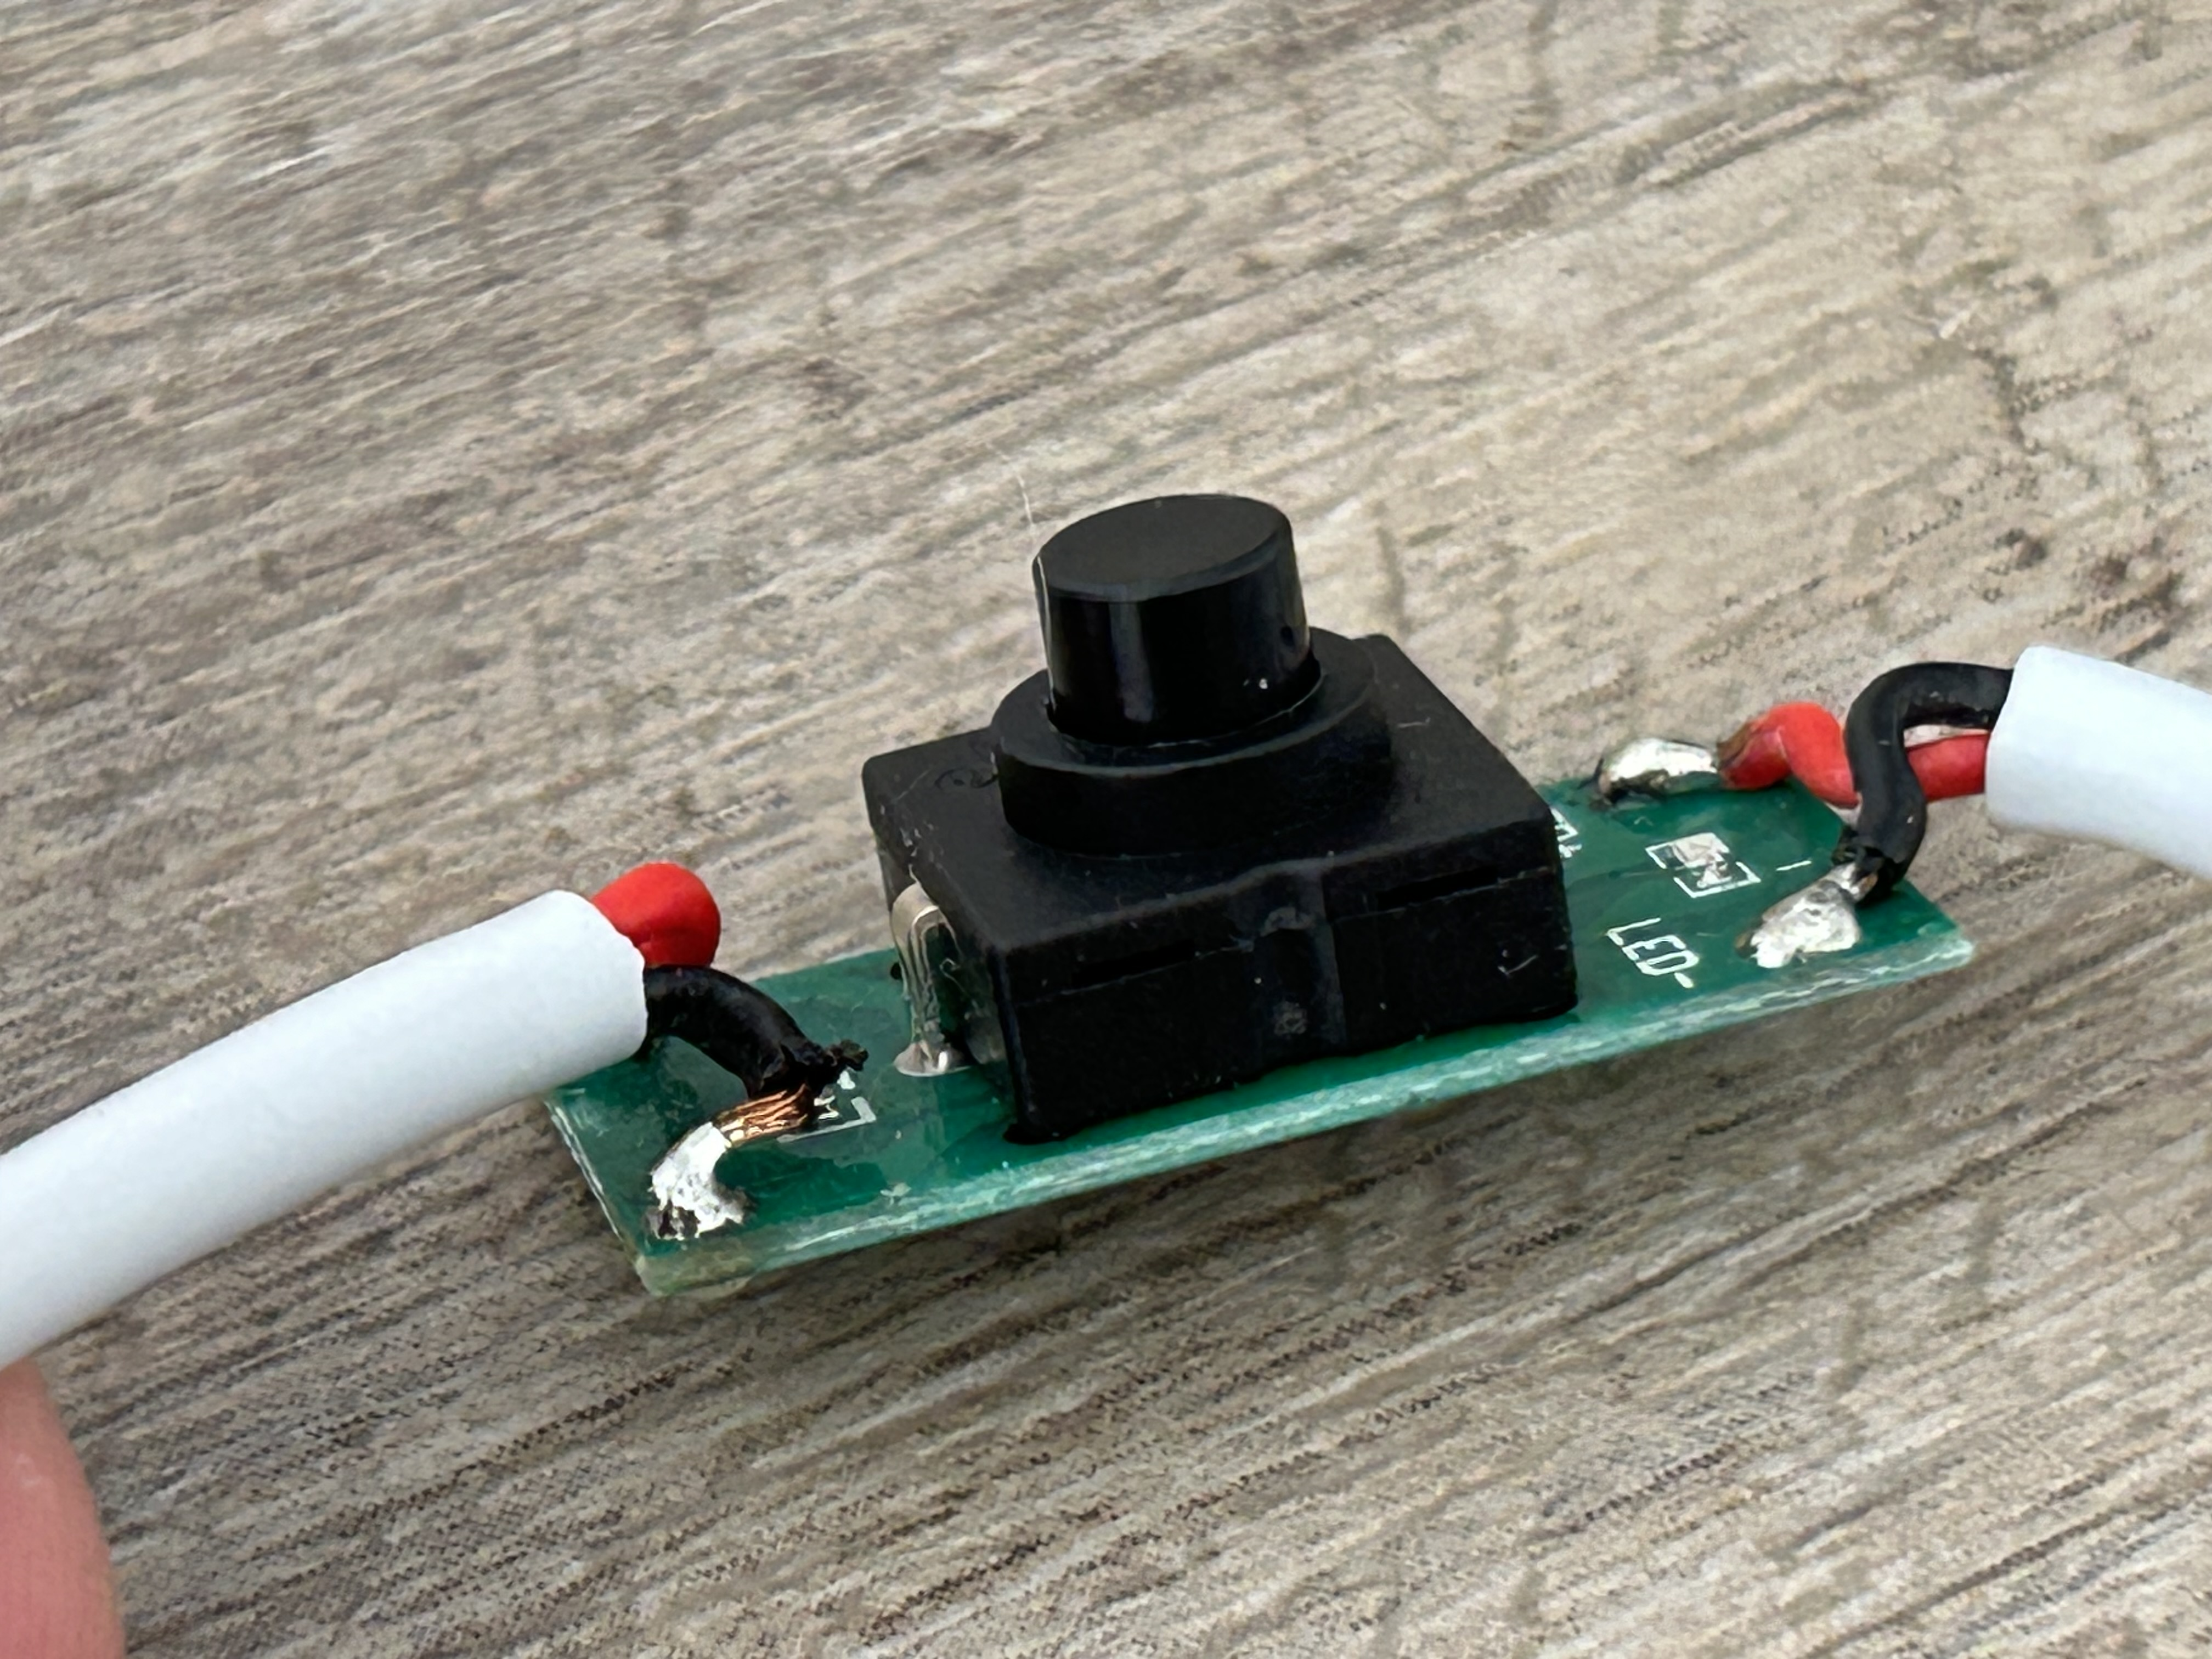
\includegraphics[height=5 cm]{texs/Part1/chapter4/image/d00.jpg}
    \caption{Power Switch}
    \label{fig:power_switch}
\end{figure}

\subsubsection{Camera Protection}
Figure \ref{fig:camera_position} shows the original position of the camera component. As seen in the figure, the camera is seamlessly integrated into the device's body, with the lens protruding slightly.

However, this design does pose a potential risk. If the device is inadvertently placed with the lens side facing a surface, it could get damaged, severely affecting its performance.

\begin{figure}[!ht]
    \centering
    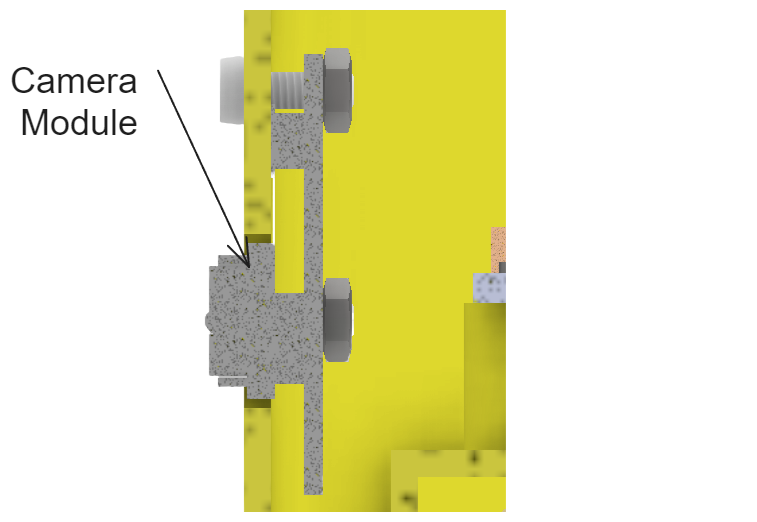
\includegraphics[height=5 cm]{texs/Part1/chapter4/image/d1.png}
    \caption{Position of the camera component}
    \label{fig:camera_position}
\end{figure}

To address this concern, we have incorporated a 3 mm high bump (as seen in Figure \ref{fig:detail_camera_protect}) as a preventative measure. The bump is strategically positioned to lift the camera lens above surfaces, preventing direct contact.

\begin{figure}[!ht]
    \centering
    \begin{subfigure}[c]{0.47\textwidth}
        \begin{minipage}{\textwidth}
            \centering
            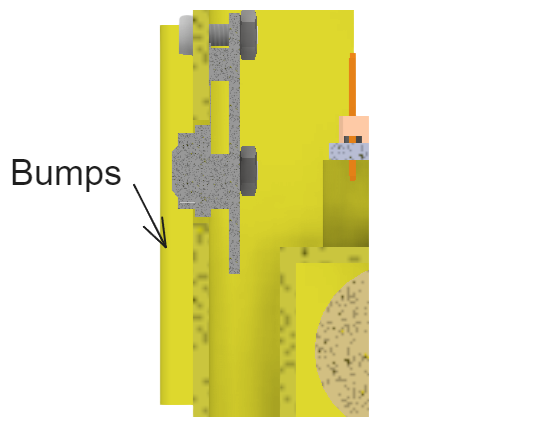
\includegraphics[height=4 cm]{texs/Part1/chapter4/image/d12.png}
        \end{minipage}
        \caption{Left View}
        \label{fig:detail_camera_left}
    \end{subfigure}
    \begin{subfigure}[c]{\textwidth}
        \begin{minipage}{\textwidth}
            \centering
            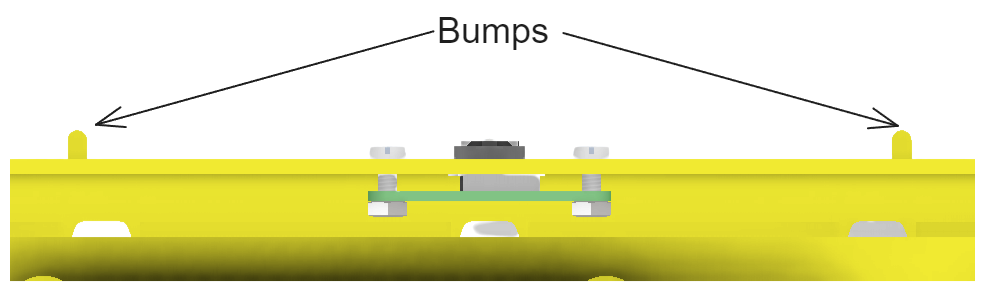
\includegraphics[width=0.75\linewidth]{texs/Part1/chapter4/image/d13.png}
        \end{minipage}
        \caption{Top View}
        \label{fig:detail_camera_top}
    \end{subfigure}
    \caption{Protective bump for camera}
    \label{fig:detail_camera_protect}
\end{figure}

\subsubsection{Screen Protection}
Similar to the camera, the screen of the device also requires protection. Similar to the camera protection, a protective bump has been incorporated around the screen perimeter to address this issue. Refer to Figure \ref{fig:detail_screen_protect} for a visual representation.

\begin{figure}[!ht]
    \centering
    \begin{subfigure}[c]{0.47\textwidth}
        \begin{minipage}{\textwidth}
            \centering
            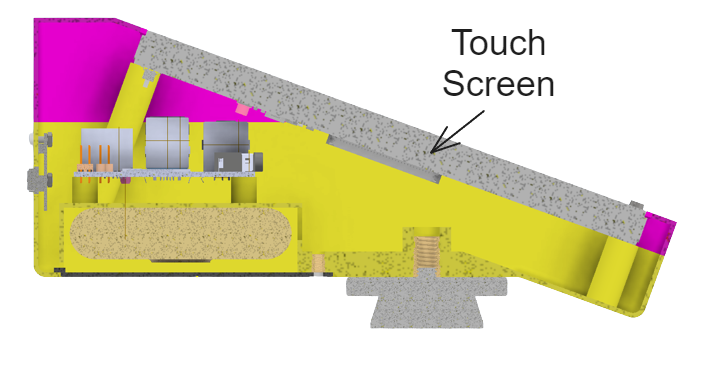
\includegraphics[height=3.5 cm]{texs/Part1/chapter4/image/d21.png}
        \end{minipage}
        \caption{Before}
        \label{fig:detail_screen_before}
    \end{subfigure}
    \begin{subfigure}[c]{0.47\textwidth}
        \begin{minipage}{\textwidth}
            \centering
            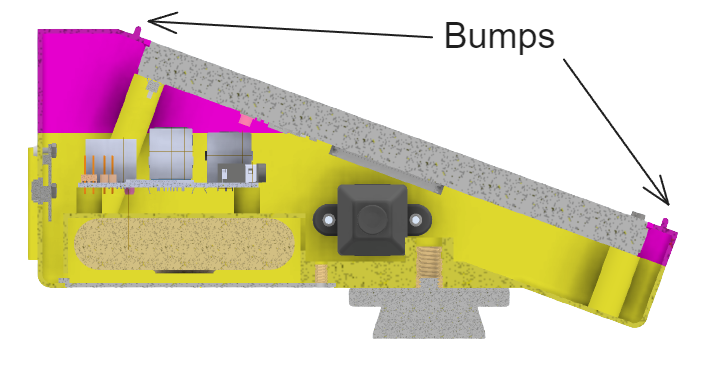
\includegraphics[height=3.5 cm]{texs/Part1/chapter4/image/d22.png}
        \end{minipage}
        \caption{After}
        \label{fig:detail_screen_after}
    \end{subfigure}
    \caption{Protective bump for screen}
    \label{fig:detail_screen_protect}
\end{figure}

\subsubsection{Column for Threaded Inserts}
Previously, in Section \ref{subsec:preliminary_design_variant_2}, we delved into utilizing threaded inserts alongside screws to firmly attach components to the body. It is crucial to note that distinct sizes of threaded inserts necessitate particular minimum wall thicknesses for the columns and hole depths to guarantee adequate engagement and steadiness. A sizing guide is provided by Ruthex threaded inserts, as shown in Table \ref{tab:threaded_inserts_sizing_guide}.

\begin{table}[!ht]
    \centering
    \begin{tabular}{|c|c|c|c|}
        \hline
        \textbf{Thread Size} & \textbf{Hole size (mm)} & \textbf{Min. thickness (mm)} & \textbf{Min. height (mm)} \\ \hline
        M2.5                 & 4                       & 1.6                          & 6.7                       \\ \hline
        1/4"                 & 8                       & 3.3                          & 13.7                      \\ \hline
    \end{tabular}
    \caption{Sizing guide for threaded inserts \cite{ruthex1}\cite{ruthex2}}
    \label{tab:threaded_inserts_sizing_guide}
\end{table}


\subsubsection{LAN Port}
To enable easier maintenance of the Raspberry Pi, a Local Area Network (LAN) port is added to the device, which enables the Raspberry Pi to be accessed directly without disassembly. This strategic integration allows seamless connectivity, enabling direct access to the Raspberry Pi's functionalities and resources over a local network. Figure \ref{fig:lan_port} shows the LAN port.

The LAN port, illustrated in Figure \ref{fig:lan_port}, is positioned on the side of the device (as shown in Figure \ref{fig:lan_port_position}), making it easy for users to perform maintenance tasks.

\begin{figure}[!ht]
    \centering
    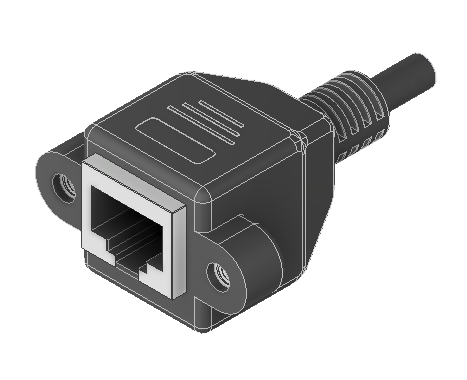
\includegraphics[height=5 cm]{texs/Part1/chapter4/image/d31.png}
    \caption{The LAN port}
    \label{fig:lan_port}
\end{figure}

\begin{figure}[!ht]
    \centering
    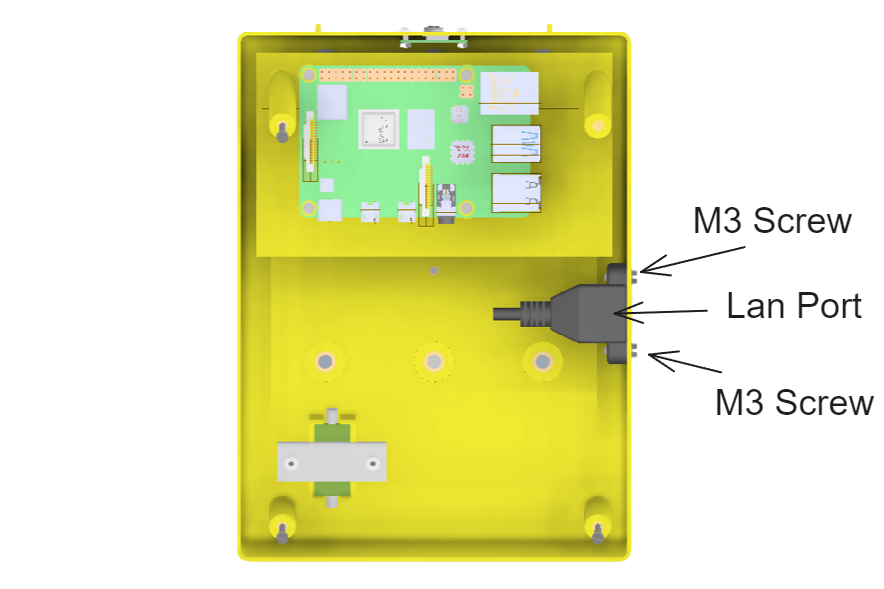
\includegraphics[height=5 cm]{texs/Part1/chapter4/image/d32.png}
    \caption{Position of the LAN port}
    \label{fig:lan_port_position}
\end{figure}

\subsubsection{Color Scheme}
The selection of colors is crucial in making the product visually appealing, especially since the target market is the police force. To achieve this, we utilized the German police logo for inspiration, as shown in Figure \ref{fig:polizei_logo}. The predominant color of blue in the logo is used as the primary color for the device. Additionally, we used yellow from the logo as the color for the handle grip and white for the device's top cover. Figure \ref{fig:color_scheme} shows the device preview with the recolor.

\begin{figure}[ht!]
    \centering
    
\includegraphics[height=5 cm]{texs/Part1/chapter4/image/polizei.jpg}
    \caption{Germany Police Logo \cite{bundespolizei}}
    \label{fig:polizei_logo}
\end{figure}

\begin{figure}[ht!]
    \centering
    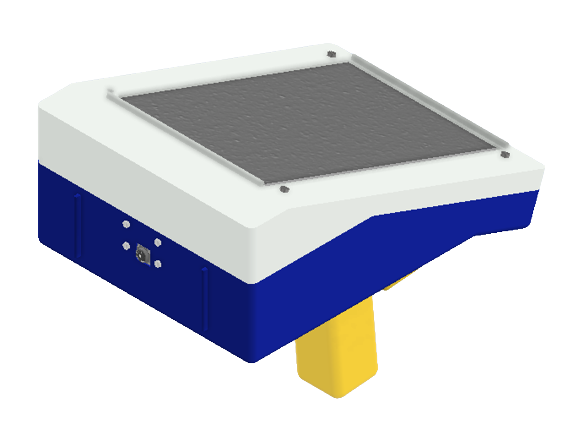
\includegraphics[height=9 cm]{texs/Part1/chapter4/image/d41.png}
    \caption{Result of recolor}
    \label{fig:color_scheme}
\end{figure}


